% 1977 年河北卷第 2 题：直径、切线与平行弦
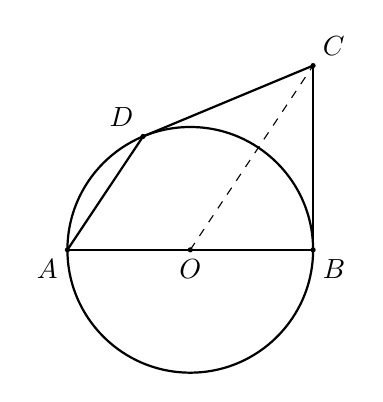
\begin{tikzpicture}[scale=0.78,>=stealth]
  \coordinate (O) at (0,0);
  \coordinate (A) at (-2,0);
  \coordinate (B) at (2,0);
  \coordinate (C) at (2,3);
  \coordinate (D) at (-0.769,1.846);
  \draw[thick] (O) circle (2);
  \draw[thick] (A)--(B);
  \draw[thick] (B)--(C);
  \draw[thick] (A)--(D);
  \draw[thick] (D)--(C);
  \draw[dashed] (O)--(C);
  \fill (O) circle (1.2pt) node[below] {$O$};
  \fill (A) circle (1.2pt) node[below left] {$A$};
  \fill (B) circle (1.2pt) node[below right] {$B$};
  \fill (C) circle (1.2pt) node[above right] {$C$};
  \fill (D) circle (1.2pt) node[above left] {$D$};
\end{tikzpicture}
